\begin{ledgroupsized}[r]{120mm}
\footnotesize
\pstart
\noindent\textbf{\"{U}berlieferung:}
\pend
\end{ledgroupsized}
%
\begin{ledgroupsized}[r]{114mm}
\footnotesize
\pstart
\parindent -6mm
\makebox[6mm][l]{\textit{L}}Konzept: LH XXXV 14, 2 Bl. 114-115. 1 Bog. 2\textsuperscript{o}. 2 \nicefrac{4}{5} S. auf Bl. 114~r\textsuperscript{o} bis Bl. 115~r\textsuperscript{o}. Das letzte Fünftel von Bl. 115~r\textsuperscript{o} sowie Bl. 115~v\textsuperscript{o} überliefern den Anfang von N. 50. Auf Bl. 115~v\textsuperscript{o} findet sich zudem N. 80.
\\Cc 2, Nr. 941 B
\pend
\end{ledgroupsized}
%\normalsize
\vspace*{5mm}
\begin{ledgroup}
\footnotesize
\pstart
\noindent
\footnotesize{\textbf{Datierungsgr\"{u}nde}: Das vorliegende Stück N.~9 %?? = ex 10 = LH 35.14.02, 114-115
besteht nur scheinbar aus Exzerpten aus John Wallis' Abhandlung \cite{00301}\textit{Mechanica sive De motu} (2 Bde, London 1670-1671).
Leibniz entwickelt in diesem Stück vielmehr eigenständige Überlegungen, die von seiner Auseinandersetzung mit Wallis' Traktat herrühren.
In dieser Hinsicht dürfte N.~9 %?? = ex 10 = LH 35.14.02, 114-115
inhaltlich -- und vermutlich auch zeitlich -- mit Leibniz' Exzerpten aus Wallis' \textit{Mechanica} zusammenhängen,
die in N.~8 %?? = ex 9 = LH 35.14.02, 117-124
überliefert sind. Leibniz' Marginalie zur Überschrift in N.~9 %?? = ex 10 = LH 35.14.02, 117-124
lässt sich demnach als eine Anspielung auf die Kritiken begreifen, die in N.~8 %?? = ex 9 = LH 35.14.02, 117-124
formuliert werden (siehe oben, S.~\refpassage{LH35,14,02_121r_ref-1}{LH35,14,02_121r_ref-2};
S.~\refpassage{LH35,14,02_121r_ref-3}{LH35,14,02_121r_ref-4};
S.~\refpassage{LH35,14,02_121r_ref-5}{LH35,14,02_121r_ref-6}).
\newline\hspace*{6mm}%
Das Stück N.~9 %?? = ex 10 = LH 35.14.02, 114-115
befindet sich zusammen mit dem Anfang von N.~50 %?? LH 35.14.02, 112-115
(d.h. von Leibniz' Exzerpten aus Edme Mariottes \cite{00311}\textit{Traité de la percussion}, Paris 1673)
auf ein und demselben Bogen, wobei N.~50 %?? LH 35.14.02, 112-115
unmittelbar an das Ende von N.~9 %?? = ex 10 = LH 35.14.02, 114-115
anschließt. Daher ist anzunehmen, dass N.~9 %?? = ex 10 = LH 35.14.02, 114-115
kurz oder unmittelbar vor dem auf die letzten Monate 1674 datierbaren Stück N.~50 %?? LH 35.14.02, 112-115
entstanden ist.
Aus dem angeführten Grund ist die Datierung von N.~50 auch für das vorliegende Stück N.~9 %?? = ex 10 = LH 35.14.02, 114-115
zu übernehmen.}
\pend
\end{ledgroup}
%
%%%%%%%%%% HIER BEGINNT BLATT 114r.
%
\vspace{5.0mm}
\count\Afootins=1500
\count\Bfootins=1500
\count\Cfootins=1500
\pstart
\noindent
[114~r\textsuperscript{o}]
\pend
\pstart
\centering
\edtext{Excerpta ex Wallisio\protect\index{Namensregister}{\textso{Wallis} (Wallisius), John 1616-1703}
cogitatis obiter occurrentibus aucta.}{\lemma{}\Afootnote{\textit{Darunter:} Imo coepi excerpere,
sed vidi in progressu,
vix quicquam ab eo exacte demonstrari.\vspace{-8mm}}}\label{LH35,14,02_114r_ref-1}
\pend
\vspace{0.5em}
\pstart
\noindent
\edlabel{35,14,02_114r_01}\edtext{}{{\xxref{35,14,02_114r_01}{35,14,02_114r_02}}\lemma{\textso{Motus} [...] rationis}\Cfootnote{Die Definitionen orientieren sich teilweise an J. \textsc{Wallis}, \textit{Mechanica}, pars I, cap. 1, London 1670-1671, S. 1-8\cite{00301} (\textit{WO} I, S. 575-579\cite{01008}).}}\textso{Motus }est mutatio
\edtext{loci.\\
\hspace*{7,5mm}%
\textso{Velocitas}\protect\index{Sachverzeichnis}{velocitas}\textso{ }est quantitas motus id est quantitas loci qui mutatus
\edtext{sive decursus}{\lemma{sive decursus}\Bfootnote{\textit{erg. L}}}
est certo quodam tempore dato.}{\lemma{loci.}\Bfootnote{%
\textit{(1)}\ \textso{Velocitas }est quantitas loci et temporis in motu
\textit{(2)}\ \textso{Velocitas} [...] dato
\textit{L}}}\\
\hspace*{7,5mm}%
\textso{Conatus}\protect\index{Sachverzeichnis}{conatus}\textso{ }est initium
\edtext{motus.\\
\hspace*{7,5mm}%
\textso{Impetus}\protect\index{Sachverzeichnis}{impetus}\textso{ }est quantitas conatus.\\
\hspace*{7,5mm}%
\textso{Vis}\protect\index{Sachverzeichnis}{vis}\textso{ }est}{\lemma{motus.}\Bfootnote{%
\textit{(1)}\ \textso{Vis} 
\textit{(2)}\ initium
\textit{(3)}\ conatus est
\textit{(4)} \textso{Impetus} [...] \textso{Vis} est
\textit{L}}}
impetuum conspirantium summa.
Hinc fit ut vulgo dicant vim fieri 
ex ductu magnitudinis corporis\protect\index{Sachverzeichnis}{corpus} in impetum.
Quoniam scilicet tot intelligi possunt impetus quot 
corporis partes.
\pend
\count\Afootins=1200
\count\Bfootins=1200
\count\Cfootins=1200
\pstart
%\hspace*{7,5mm}%
\textso{Pondus}\protect\index{Sachverzeichnis}{pondus}\textso{ }est vis corporum 
quorum conatus est versus centrum terrae, seu vis gravium.\\
\hspace*{7,5mm}%
\textso{Resistentia}\protect\index{Sachverzeichnis}{resistentia}\textso{ }tanta est,
quantus est conatus, cujus impeditur motus.\\
\hspace*{7,5mm}%
\textso{Onus}\protect\index{Sachverzeichnis}{onus}\textso{ }est pondus gravis
\edtext{movendi ab extrinseco, sive aliter}{\lemma{movendi}\Bfootnote{%
\textit{(1)}\ aliter
\textit{(2)}\ ab [...] aliter
\textit{L}\hspace{-2mm}}}
quam suapte sponte iret.
Itaque onus est resistentiae species.\\
\hspace*{7,5mm}%
\textso{Directio}\protect\index{Sachverzeichnis}{directio}\textso{ }est recta tangens lineam
in qua fit conatus vel
\edtext{motus.\\
\hspace*{7,5mm}%
\textso{Obliquitas}\protect\index{Sachverzeichnis}{obliquitas}\textso{ }est angulus directionis motus,
ad directionem\protect\index{Sachverzeichnis}{directio} conatus;}{\lemma{motus.}\Bfootnote{%
\textit{(1)} \textso{Declivitas} est quantitas anguli directionis ad ang
\textit{(2)} \textso{Obliquitas} [...] conatus
\textit{L}\hspace{-4mm}}} 
orta a \edtext{figura superficiei corporis motui in conatum directo resistentis.}{\lemma{figura}\Bfootnote{%
\textit{(1)}\ corporis solidi
\textit{(2)}\ superficiei corporis
\textit{(a)}\ directioni
\textit{(b)}\ motui [...] resistentis
\textit{L}\hspace{-4mm}}}\\
\hspace*{7,5mm}%
\textso{Motus directus }est,
cum linea conatus et motus coincidunt.\\
\hspace*{7,5mm}%
\textso{Gravitas}\protect\index{Sachverzeichnis}{gravitas}\textso{ }appellari potest in staticis generalibus:
Conatus ad planum in recta angulos 
ad planum rectos faciente, sive in linea brevissima.\\
\hspace*{7,5mm}%
%%%%%%%%%
Declivitas\protect\index{Sachverzeichnis}{declivitas}
(sive Acclivitas\protect\index{Sachverzeichnis}{acclivitas} in \edtext{ascensu)
ratio}{\lemma{ascensu)}\Bfootnote{%
\textit{(1)}\ quantitas
\textit{(2)}\ ratio
\textit{L}\hspace{-3mm}}}
rectae $\displaystyle AC$ ad rectam $\displaystyle AB$ seu 
ratio rectae ex puncto dato ad planum ductae ad [brevissimam].\edtext{}{\lemma{}\Bfootnote{\hspace{-2mm}brevissimum \textit{L ändert Hrsg.}}}\\
\hspace*{7,5mm}%
\textso{Obliquitas}\protect\index{Sachverzeichnis}{obliquitas}\textso{ }est quantitas anguli $\displaystyle BAC$.\\
\hspace*{7,5mm}%
\textso{Inclinatio}\protect\index{Sachverzeichnis}{inclinatio}\textso{ }quantitas anguli $\displaystyle ACB$.
Antecedentem per consequens divisum esse indicem
rationis.\edlabel{35,14,02_114r_02}\\
\hspace*{7,5mm}%
\edtext{$\displaystyle\infty$ est signum infiniti\protect\index{Sachverzeichnis}{signum infiniti}
apud Wallisium\protect\index{Namensregister}{\textso{Wallis} (Wallisius), John 1616-1703}.}{%
\lemma{$\displaystyle\infty$ [...] Wallisium}%
\Cfootnote{\cite{00301}a.a.O., S. 12 (\textit{WO} I, S. 582\cite{01008}). Siehe auch J. \textsc{Wallis}, \cite{00302}\textit{De sectionibus conicis}, Oxford 1655, S. 4 (\textit{WO} I, S. 297).}}\\
\hspace*{7,5mm}%
\edtext{Effectus\protect\index{Sachverzeichnis}{effectus} sunt causis suis adaequatis\protect\index{Sachverzeichnis}{causa adaequata} proportionales seu \protect\rule[-4mm]{0mm}{10mm}$\displaystyle \frac{C}{E} \sqcap \frac{(C)}{(E)}\sqcap \frac{rC}{rE}$.}{\lemma{Effectus [...] proportionales}\Cfootnote{\cite{00301}J. \textsc{Wallis}, \textit{Mechanica}, pars I, cap. 1, London 1670-1671, prop. VII, S. 15 (\textit{WO} I, S. 584\cite{01008}).}}
\pend
\vspace{0.5em}
\pstart
\centering
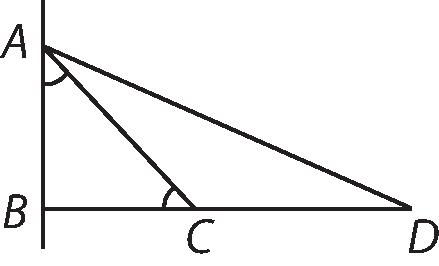
\includegraphics[trim = 0mm 0mm 0mm 0mm, clip, width=0.27\textwidth]{images/LH035,14,02_114r-d1.pdf}\\
\noindent
\centering
[\textit{Fig. 1}] % \caption{Bildbeschreibung}
\pend
\newpage
\pstart
%\vspace*{1.5em}% PR: Rein provisorisch!!
\hspace*{9mm}
\begin{minipage}[t]{0.26\textwidth}
%\hspace*{5mm}
%\centering
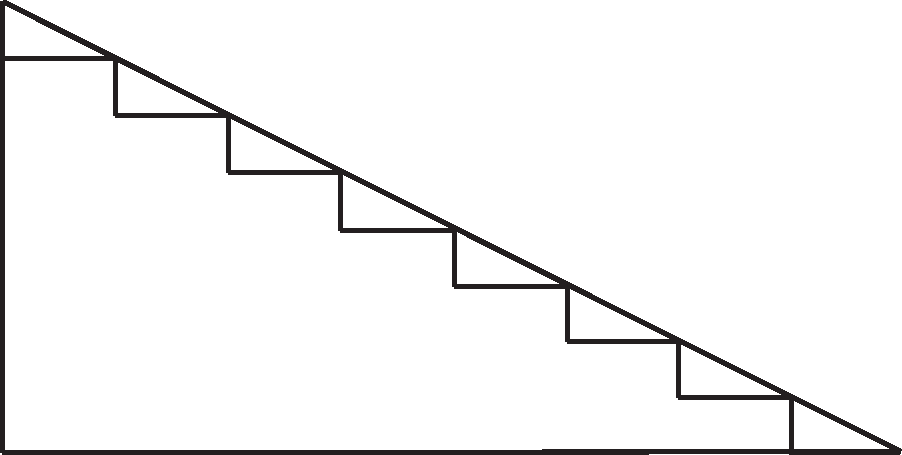
\includegraphics[width=0.98\textwidth]{images/LH035,14,02_114r-d2.pdf}\\ \\
\noindent
\centering
%\hspace{15mm}
[\textit{Fig. 2, gestrichen}]
\end{minipage}
\hspace*{25mm}
\begin{minipage}[t]{0.26\textwidth}
%\hspace*{-5mm}
%\centering
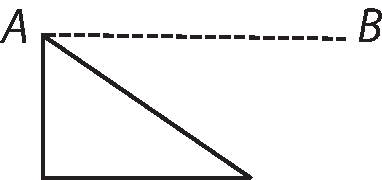
\includegraphics[width=0.98\textwidth]{images/LH035,14,02_114r-d3.pdf}\\ \\
\noindent
\centering
%\hspace{-5mm}
[\textit{Fig. 3}]
\end{minipage}
% \hspace*{13mm} [\textit{Fig. 2, gestrichen}]\hspace*{46mm} [\textit{Fig. 3}]
\pend
\count\Afootins=1200
\count\Bfootins=1200
\count\Cfootins=1200
\vspace{2.5em}
\pstart
\edtext{Theorema meum.}{\lemma{}\Afootnote{\textit{Am Rand:} Haec et sequentia a me.}}
\setline{1}Grave\protect\index{Sachverzeichnis}{grave} minore celeritate\protect\index{Sachverzeichnis}{celeritas}
pervenit ad terram in plano inclinato\protect\index{Sachverzeichnis}{planum inclinatum},
quam in perpendiculari:
nam alioquin nihil impediret obstaculum,
sed potius augeret celeritatem.
Faceret enim ut alia linea major eodem tempore percurreretur;
quod absurdum.
Deinde pone inclinatum eodem tempore absolvi,
fingatur inclinatio\protect\index{Sachverzeichnis}{inclinatio} plani $\displaystyle AB$ infinite parva,
non quiescet in ea grave\protect\index{Sachverzeichnis}{grave},
sed infinita celeritate\protect\index{Sachverzeichnis}{celeritas} movebitur,
quod est \edtext{absurdum.
Sed ut ista exactius comprehendantur, ita concipiemus.}{\lemma{absurdum.}\Bfootnote{%
\textit{(1)}\ Demonstrandum est:
\textit{(a)}\ eandem esse celeritatem gravis descendentis in plano inclinato\protect\index{Sachverzeichnis}{planum inclinatum}, quae est descendentis
\textit{(b)}\ eundem esse impetum gravis descendere incipientis in plano inclinato, quae [\textit{sic}] est descendere incipientis in perpendiculo.
Quod ita ostenditur:
Quia eadem est quae ante vis motrix\protect\index{Sachverzeichnis}{vis motrix},
causa scilicet gravitatis\protect\index{Sachverzeichnis}{causa gravitatis}.
Eadem autem vis in idem corpus agens
\textit{(aa)}\ non p
\textit{(bb)}\ eundem producit effectum\protect\index{Sachverzeichnis}{effectus}.
Sane non erit major celeritas, ut patet, sed nec minor.
\textit{(2)}\ Sed ut [...] concipiemus.
\textit{L}}}
\pend
\pstart
\edtext{Ostensum a me}{\lemma{}\Afootnote{\textit{Am Rand:} Haec a me inventa.\vspace{-5mm}}}
\edtext{alibi}{\lemma{alibi}\Cfootnote{\cite{01156}\textit{LSB} VI, 2 N. $42_4$, S. 281.16-18.}}
est omnem conatum\protect\index{Sachverzeichnis}{conatus} in una recta
intelligi posse in aliis omnibus[,]
ut $\displaystyle AB$ etiam intelligi posse excerceri in $\displaystyle AC$
ob compositionem conatuum in $\displaystyle AC$ et $\displaystyle AD,$
sed ideo motus tardior in $\displaystyle AC$ conatus quam in $\displaystyle AB.$
Quod nobis obstat.
\pend
\pstart
Jam si gravitatem\protect\index{Sachverzeichnis}{gravitas} intelligamus proficisci[,]
cogitemus a causa\protect\index{Sachverzeichnis}{causa} quadam corpori $\displaystyle E$ continuos ictus ex linea $\displaystyle GE,$
perpendiculari ad $\displaystyle FE$ horizontalem, infligenti,
futura est profecto celeritas excipientis $\displaystyle E$,
non longe minor quam celeritas impingentis,
quia non nisi partem ictus\protect\index{Sachverzeichnis}{ictus}, longe scilicet minorem, excipiet. 
Nimirum si sit recta $\displaystyle AD,$ ad rectam $\displaystyle AC$ ut $\displaystyle b$ ad $\displaystyle c,$
etiam celeritas conatus\protect\index{Sachverzeichnis}{celeritas conatus} in $\displaystyle AC$
[ad]\edtext{}{\lemma{ad}\Bfootnote{\textit{erg. Hrsg.}}}
celeritatem conatus in $\displaystyle AD$ eodem modo 
\pend
\pstart
\begin{minipage}[c]{0.32\textwidth}
%\hspace*{5mm}
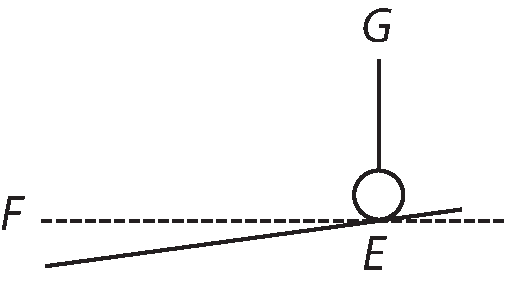
\includegraphics[width=0.98\textwidth]{images/LH035,14,02_114r-d4.pdf}
%\\ \\
%\noindent\centering[\textit{Fig. 4}]
\end{minipage}
\hspace*{26mm}
\begin{minipage}[c]{0.3\textwidth}
\hspace*{-5mm}
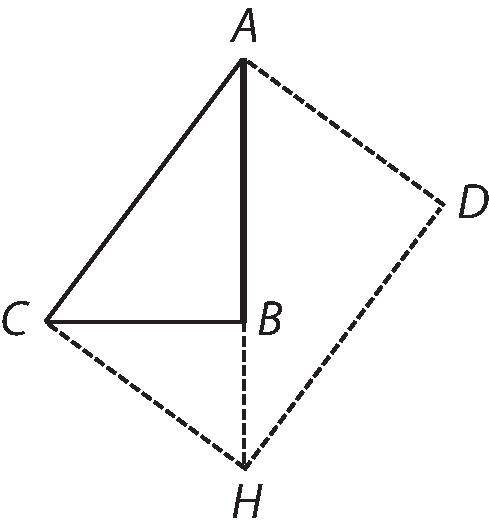
\includegraphics[width=0.98\textwidth]{images/LH035,14,02_114r-d5.pdf}
%\\ \\
%\noindent\centering[\textit{Fig. 5}]
\end{minipage}
%\vspace*{2mm}
\setline{1}\rule[-4mm]{0mm}{8mm}\hspace*{14mm} [\textit{Fig. 4}]\hspace*{54mm} [\textit{Fig. 5}]\\
\\
%\vspace*{2em}
\noindent
\centering
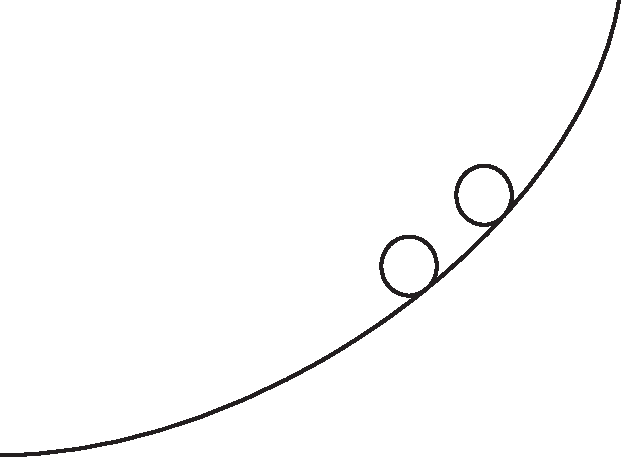
\includegraphics[trim = 0mm -3mm 0mm 0mm, clip, width=0.30\textwidth]{images/LH035,14,02_114r-d6.pdf}\\
\noindent \centering [\textit{Fig. 6}]
\pend
\vspace{1.5em}
\pstart\noindent
erit. 
\setline{1}Celeritas\protect\index{Sachverzeichnis}{celeritas} autem in recta
\edtext{$\displaystyle AB$ est}{\lemma{$\displaystyle AB$}\Bfootnote{%
\textit{(1)}\ erit
\textit{(2)}\ est
\textit{L}}}
ad celeritatem in recta $\displaystyle AC$,
ut $\displaystyle AH$ \edtext{ad $\displaystyle AC.$
(:~Est autem ipsius $\displaystyle AH$ ratio ad $\displaystyle AB$ varia.}{\lemma{ad $\displaystyle AC.$}\Bfootnote{%
\textit{(1)}\ cujus $\displaystyle AH$ ratio ad $\displaystyle AB$ variat.
Est autem $\displaystyle AH$ semper ipsius $\displaystyle AB$ dupla,
\textit{(2)}\ (:~Est [...] varia.
\textit{L}}}
Haec contemplatio cum sit plane nova, nec quod sciam satis a quoquam excussa; satis memorabilis videtur.~:)
Jam ob Triangula $\displaystyle ACH$ et $\displaystyle ABC$ similia est $\displaystyle AH$ ad $\displaystyle AC$ ut $\displaystyle AC$ ad $\displaystyle AB$.
Erit ergo celeritas in recta $\displaystyle AB$ quae sola excipitur[,]
ad celeritatem\protect\index{Sachverzeichnis}{celeritas} in recta $\displaystyle AC$ quae sola excipitur[,]
ut $\displaystyle AC$ ad $\displaystyle AB$
seu in reciproca rectarum ratione:
ac proinde conatus\protect\index{Sachverzeichnis}{conatus} descendendi in recta $\displaystyle AC$ inclinata,
ad conatum descendendi in perpendiculari, $\displaystyle AB$, erit, ut
\edtext{eadem}{\lemma{eadem}\Bfootnote{\textit{erg. L}}}
$\displaystyle AB$ perpendicularis ad $\displaystyle AC$
\edlabel{35,14,02_114r_03}\edtext{}{{\xxref{35,14,02_114r_03}{35,14,02_114r_04}}\lemma{inclinatam.}\Bfootnote{%
\textit{(1)}\ Unde cum praeterea tempus
\textit{(2)}\ Si celeritas\protect\index{Sachverzeichnis}{celeritas} uniformis foret,
tempora descensuum futura sint ut lineae,
sequitur tempus quo descendatur in linea $\displaystyle AC$, fore ad tempus
quo descenditur in linea $\displaystyle AB$ in duplicata linearum ratione.
Si quidem gravitas\protect\index{Sachverzeichnis}{gravitas} oritur a causa quadam
continuis ictibus\protect\index{Sachverzeichnis}{ictus}\ \textbar\ $\displaystyle AB$ \textit{gestr.}\ \textbar\
ad horizontem perpendicularibus solicitante,
quales ictus essent effluviorum quorundam ex terra,
\textit{(3)}\ Tarditas [...] celeritatum~:).
\textit{L}}}inclinatam.
\pend
\pstart
%\vspace{0.5em}% PR: Rein provisorisch!!
\begin{minipage}[t]{0.28\textwidth}
\hspace*{10mm}
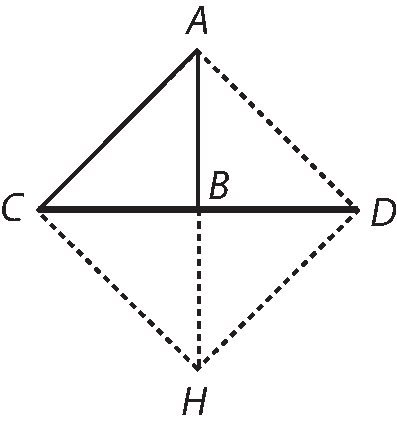
\includegraphics[trim = 0mm -3mm 0mm 0mm, clip, width=1.0\textwidth]{images/LH035,14,02_114r-d7.pdf}
%\\
%\noindent \centering [\textit{Fig. 7}]
\end{minipage}
\hspace*{38,9mm}
\begin{minipage}[t]{0.26\textwidth}
\hspace*{-5mm}
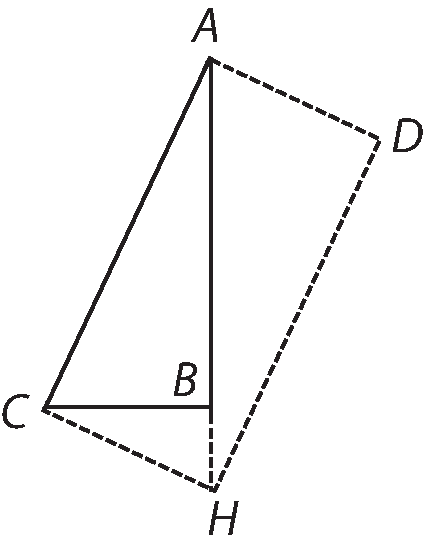
\includegraphics[trim = 0mm -3mm 0mm 0mm, clip, width=1.0\textwidth]{images/LH035,14,02_114r-d8.pdf}
%\\
%\noindent \centering [\textit{Fig. 8}]
\end{minipage}\\
%\vspace*{1mm}
\hspace*{29mm} [\textit{Fig. 7}]\hspace*{51mm} [\textit{Fig. 8}]
\pend
\vspace{2.5em}
\pstart
Tarditas\protect\index{Sachverzeichnis}{tarditas} \setline{1}in $\displaystyle AC$, est ad tarditatem in $\displaystyle AB$
ut linea $\displaystyle AC$ ad lineam $\displaystyle AB$,
id est conatus\protect\index{Sachverzeichnis}{conatus} in $\displaystyle AC$ in ea ratione est tardior conatu in $\displaystyle AB$
in qua ratione $\displaystyle AC$ est major quam $\displaystyle AB$
(:~ut scilicet directam potius adhibeamus rationem tarditatum\protect\index{Sachverzeichnis}{tarditas},
quam reciprocam celeritatum~:).%
\edlabel{35,14,02_114r_04}
Ergo et tempora quibus aequalia spatia percurruntur;
ergo et incrementa aequabilia\protect\index{Sachverzeichnis}{incrementum celeritatis}
\edtext{celeritatum\protect\index{Sachverzeichnis}{celeritas}}{\lemma{celeritatum}\Bfootnote{\textit{erg. L}\hspace{-2mm}}}
erunt ut lineae,
ergo et summae eorum erunt lineis proportionales:
Ergo cum conatus simplices\protect\index{Sachverzeichnis}{conatus simplex} sint ut in
\edtext{ratione linearum reciproca}{\lemma{ratione}\Bfootnote{%
\textit{(1)}\ linearum directa
\textit{(2)}\ linearum reciproca
\textit{L}}},
\edtext{accelerationes\protect\index{Sachverzeichnis}{acceleratio} in directa}{\lemma{accelerationes in}\Bfootnote{%
\textit{(1)}\ reciproca
\textit{(2)}\ directa
\textit{L}}};
compositione autem reciprocae et directae fiat ratio
\edtext{aequalitatis. Erunt celeritates\protect\index{Sachverzeichnis}{celeritas}}{\lemma{aequalitatis.}\Bfootnote{%
\textit{(1)}\ Erit celeritas
\textit{(2)}\ Erunt celeritates
\textit{L}}}
in fine \edtext{acquisitae, aequales}{\lemma{acquisitae,}\Bfootnote{%
\textit{(1)}\ ad celeritatem quaesitam initio
\textit{(2)}\ aequales
\textit{L}}};
ac proinde et tempora erunt ut lineae.
Quare habemus perfectam demonstrationem
\edtext{eorum quae a
Galilaeo\protect\index{Namensregister}{\textso{Galilei} (Galilaeus, Galileus), Galileo 1564-1642}
sumta sunt}{\lemma{eorum [...] sunt}\Cfootnote{G. \textsc{Galilei}, \cite{00050}\textit{Discorsi}, Leiden 1638, S. 166 (\cite{00048}\textit{GO} VIII, S. 205).\hspace{25mm}}}
eamque a priori et ex intimis motus visceribus sumtam.
Cum \edtext{Hugeniana\protect\index{Namensregister}{\textso{Huygens} (Hugenius, Ugenius, Hugens, Huguens), Christiaan 1629-1695},
sane ingeniosissima supponat
impossibile esse ut grave\protect\index{Sachverzeichnis}{grave}
vi gravitatis\protect\index{Sachverzeichnis}{vis gravitatis} altius assurgat
quam unde [deciderat]\edtext{}{\lemma{dedicerat}\Bfootnote{\textit{L ändert Hrsg.}}}
sive motum perpetuum\protect\index{Sachverzeichnis}{motus perpetuus}
existere non posse.}{\lemma{Hugeniana [...] posse}\Cfootnote{%
C. \textsc{Huygens}, \cite{00123}\textit{Horologium oscillatorium}, II, prop. VI, Paris 1673, S. 32 (\cite{00113}\textit{HO} XVIII, S. 143).}}
Quod mihi vel eo magis dubium.
Quia iisdem probabilitatis argumentis concludi posset,
nec grave\protect\index{Sachverzeichnis}{grave} eo usque assurgere posse, unde decidit.
Cujus contrarium verum, ipso demonstrante.
\pend
\newpage
\pstart
\vspace*{1.0em}
\noindent
\centering
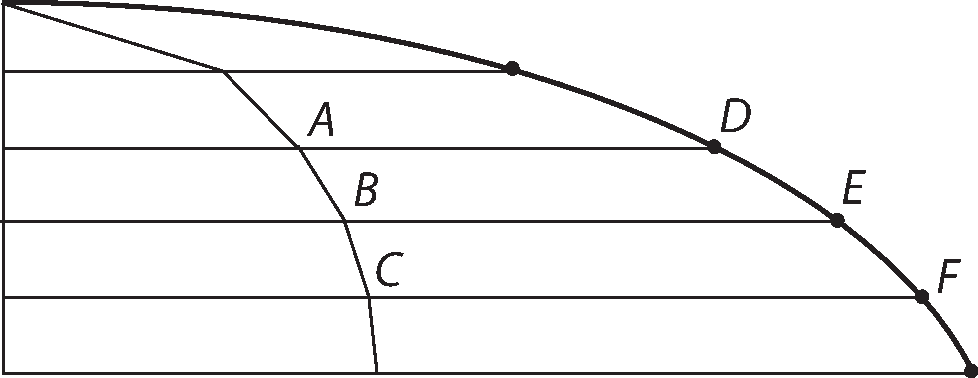
\includegraphics[trim = 0mm -3mm 0mm 0mm, clip, width=0.55\textwidth]{images/LH035,14,02_114r-d9.pdf}\\
%\vspace*{0.5em}
\noindent \centering [\textit{Fig. 9}]
\pend
\vspace*{2.5em}
\pstart
Haec \setline{1}si velis, de reciprocis rationum compositionibus aequalitatem facientibus per figuras demonstrare possis.
Pone v.g. $\displaystyle AB,$ $\displaystyle BC,$ esse ut applicatas Trianguli, $\displaystyle DE,$ $\displaystyle EF,$
esse reciprocas, seu ut applicatas Hyperbolae\protect\index{Sachverzeichnis}{hyperbola} circa
\edtext{Asymptoton\protect\index{Sachverzeichnis}{asymptotos},}{\lemma{}\Afootnote{\textit{\"{U}ber} Asymptoton: \Denarius}}
\edtext{erunt tempora quibus spatia percurruntur inclinata ad tempora quibus aequalia spatia recta,
ut reciprocae applicatarum homogeneae ipsis $\displaystyle AB$
seu ut applicatae Hyperbolae\protect\index{Sachverzeichnis}{hyperbola}
si $\displaystyle ABC$ sit recta contra celeritatum incrementa\protect\index{Sachverzeichnis}{incrementum celeritatis},
in ratione directa.}{\lemma{erunt}\Bfootnote{%
\textit{(1)}\ ergo
\textit{(2)}\ tempora
\textit{(a)}\ ut
\textit{(aa)}\ Triang
\textit{(bb)}\ appli
\textit{(b)}\ quibus spatia [...] tempora quibus
\textit{(aa)}\ recta
\textit{(bb)}\ aequalia spatia recta, ut
\textit{(aaa)}\ applicatae trianguli
\textit{(bbb)}\ reciprocae [...] ipsis $\displaystyle AB$
\textit{(aaaa)}\ Contra spatia
\textit{(aaaaa)}\ quae aequalibus temporibus percurruntur, sunt ut
\textit{(bbbbb)}\ ipsa sunt
\textit{(bbbb)}\ seu ut [...] recta contra 
\textit{(aaaaa)}\ tempora
\textit{(bbbbb)}\ celeritates
\textit{(ccccc)}\ celeritatum incrementa,
\textit{(aaaaa-a)}\ ut $\displaystyle\bigtriangledown$\textsuperscript{la}. Ergo
\textit{(bbbbb-b)}\ in ratione directa.
\textit{L}}}
Ergo hinc ratio \edtext{aequalitatis.
%
[114~v\textsuperscript{o}]\\%%%%%%%%%% HIER BEGINNT BLATT 114v.
%
\hspace*{7,5mm}%
Conatus}{\lemma{aequalitatis.}\Bfootnote{%
\textit{(1)}\ Celeritas\protect\index{Sachverzeichnis}{celeritas}
\textit{(2)}\ Conatus
\textit{L}}}
in recta $\displaystyle AC$ est ad conatum\protect\index{Sachverzeichnis}{conatus}
in \edtext{recta $\displaystyle GH$ ut $\displaystyle MB$}{\lemma{%
}\Bfootnote{recta $\displaystyle GH$\ \textbar\ est \textit{streicht Hrsg.}\ \textbar\ ut $\displaystyle MB$}}
sinus rectus ad radium $\displaystyle FB$[;]
\edtext{contra}{\lemma{contra}\Bfootnote{\textit{erg. L}}}
tempus quo percurritur $\displaystyle AC$,
est ad tempus quo percurreretur $\displaystyle GH$
ut $\displaystyle FB$ ad $\displaystyle MB$.
\pend
\pstart
Celeritas\protect\index{Sachverzeichnis}{celeritas}
\edtext{acquisita gravis\protect\index{Sachverzeichnis}{grave}
descensu ex $\displaystyle M$ in $\displaystyle N$
aequatur celeritati ejusdem gravis quaesitae descensu in}{\lemma{acquisita}\Bfootnote{%
\textit{(1)}\ ejusdem
\textit{(2)}\ gravis [...] aequatur
\textit{(a)}\ descensu
\textit{(b)}\ celeritati 
\textit{(aa)}\ qua
\textit{(bb)}\ ejusdem [...] descensu
\textit{(aaa)}\ ex
\textit{(bbb)}\ in
\textit{L}}}
arcu $\displaystyle BD,$
ut patet ex praedemonstratis.
\pend
\newpage 
%\vspace*{3.5em}% PR: Rein provisorisch!
\pstart
\begin{minipage}[t]{0.33\textwidth}
\hspace*{5mm}
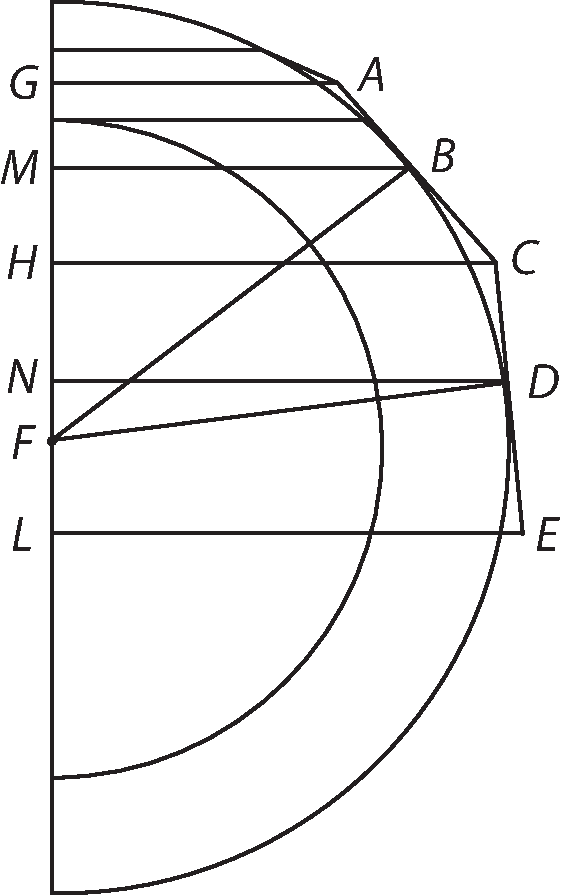
\includegraphics[trim = 0mm -3mm 0mm 0mm, clip, width=0.99\textwidth]{images/LH035,14,02_114v-d1.pdf}
%\\
%\noindent \centering [\textit{Fig. 10}]
\end{minipage}
\hspace*{26,9mm}
\begin{minipage}[t]{0.3\textwidth}
%\hspace*{-5mm}
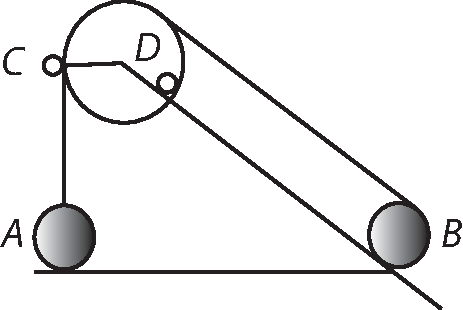
\includegraphics[trim = 0mm -3mm 0mm 0mm, clip, width=0.99\textwidth]{images/LH035,14,02_114v-d2.pdf}
%\\
%\noindent \centering [\textit{Fig. 11}]
\end{minipage}\\
%\vspace*{1mm}
\hspace*{28mm} [\textit{Fig. 10}]\hspace*{51mm} [\textit{Fig. 11}]
\pend
\vspace*{2.5em}
\pstart
Sed \setline{1}etsi celeritates sint aequales,
vires\protect\index{Sachverzeichnis}{vis} tamen[,]
id est celeritates aestimatae in perpendiculari[,]
non ideo erunt aequales;
Pone enim duo corpora $\displaystyle A.$ $\displaystyle B$ in aequilibrio esse,
pendereque ex fune trochleae circumplicato[,] alterum liberum $\displaystyle A,$
alterum plano inclinato\protect\index{Sachverzeichnis}{planum inclinatum} innitens $\displaystyle B,$
ea \edtext{magnitudinum}{\lemma{}\Afootnote{\textit{Über} magnitudinum: $\displaystyle\infty$}} ratione,
quae \edtext{sit portionum ex lineis per duas horizontales abscissarum reciproca.}{\lemma{sit}\Bfootnote{%
\textit{(1)}\ linearum
\textit{(2)}\ portionum ex lineis
\textit{(a)}\ inter
\textit{(b)}\ per duas
\textit{(aa)}\ perpendicul
\textit{(bb)}\ horizontales
\textit{(aaa)}\ comprehensarum
\textit{(bbb)}\ abscissarum reciproca
\textit{L}}}
\edtext{Pone jam}{\lemma{Pone}\Bfootnote{%
\textit{(1)}\ enim
\textit{(2)}\ jam
\textit{L}}}
duo alia corpora $\displaystyle C$ et $\displaystyle D,$
alterum in recta $\displaystyle CA,$
alterum in recta $\displaystyle DB$ inclinata,
illud corpori $\displaystyle A,$ hoc corpori $\displaystyle B$
\edtext{impingere, erunt celeritates\protect\index{Sachverzeichnis}{celeritas}}{\lemma{impingere,}\Bfootnote{%
\textit{(1)}\ manifestum est celeritates in
\textit{(2)}\ erunt celeritates
\textit{L}}} utique
\edtext{aequales, attamen ictus\protect\index{Sachverzeichnis}{ictus}
quos inter se invicem exercebunt, non erunt}{\lemma{aequales,}\Bfootnote{%
\textit{(1)}\ itaque erunt
\textit{(2)}\ attamen [...] erunt
\textit{L}}} aequales,
sed in reciproca linearum ratione,
prorsus ut [vires]\edtext{}{\lemma{vis}\Bfootnote{\textit{L ändert Hrsg.}}}
\edtext{simplices.\protect\index{Sachverzeichnis}{vis simplex}}{\lemma{%
}\Bfootnote{simplices.\ \textbar\ Sunt ergo \textit{gestr.}\ \textbar\ \textit{L}}}
\pend
\newpage
%\vspace*{2.5em}% PR: Rein provisorisch !!!
\pstart
\noindent
\centering
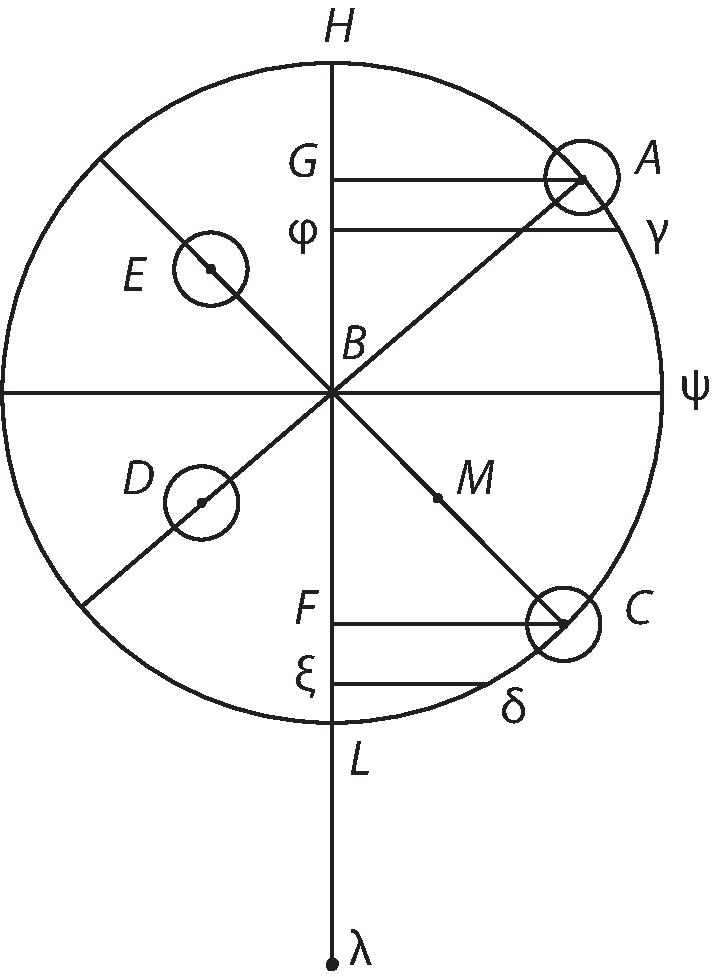
\includegraphics[trim = 0mm -3mm 0mm 0mm, clip, width=0.44\textwidth]{images/LH035,14,02_114v-d3.pdf}\\
\noindent \centering [\textit{Fig. 12}]\label{LH35,14,02_114v_ref-1}
\pend
%\newpage% PR: Rein provisorisch !!!
\vspace{1.5em}
\pstart
Si \setline{1}angulus $\displaystyle ABC$ rectus
erit \edtext{$\displaystyle GF\, \sqcap\, GA + FC$.
Sunto pondera\protect\index{Sachverzeichnis}{pondus}}{\lemma{$\displaystyle FC$.}\Bfootnote{%
\textit{(1)}\ Vis autem pon
\textit{(2)}\ Sunto pondera
\textit{L}}}
$\displaystyle 4,$ $\displaystyle A,$ $\displaystyle C,$ $\displaystyle D,$ $\displaystyle E$ aequalia,
rectaeque $\displaystyle BC,$ $\displaystyle BD$
\edtext{aequales, constat}{\lemma{aequales,}\Bfootnote{%
\textit{(1)}\ utique
\textit{(2)}\ constat
\textit{L}}}
ex demonstratis vim ponderum\protect\index{Sachverzeichnis}{vis ponderis}
$\displaystyle A + C$ in eo quem figura exhibet situ ad terram conantium,
ad vim eorum in situ absoluto esse ut $\displaystyle GF$ ad $\displaystyle HL$ diametrum
seu ut $\displaystyle AG + FC$ ad $\displaystyle AB + BC$.
Appelle vim absolutam $\displaystyle a,$
inclinatam $\displaystyle i$
erit \edtext{$\protect\rule[-4mm]{0mm}{10mm}\displaystyle\frac{i}{a}\, \sqcap\, \frac{GF}{HL}.$
A vi ponderum $\displaystyle A.\, [C]$\edtext{}{\lemma{$\displaystyle B$}\Bfootnote{ \textit{L ändert Hrsg.}}},
[auferatur]\edtext{}{\lemma{auferatur}\Bfootnote{\textit{erg. Hrsg.}}}
vis ponderum\protect\index{Sachverzeichnis}{vis ponderis} $\displaystyle E.\, D$}{\lemma{$\displaystyle\frac{i}{a}\, \sqcap\, \frac{GF}{HL}.$}\Bfootnote{%
\textit{(1)}\ inde aufera
\textit{(2)}\ ab
\textit{(3)}\ inde fieri
\textit{(4)}\ a
\textit{(5)}\ A vi ponderum $\displaystyle A.\ [C]$\ \textbar\ auferatur \textit{gestr.}\ \textbar\ vis ponderum $\displaystyle E.\ D$ 
\textit{ L}}}
quae est: $\displaystyle\frac{(i)}{(a)}\, \sqcap\, \frac{GF}{HL}.$
Erit $\protect\rule[-4mm]{0mm}{10mm}\edtext{\displaystyle i \, \sqcap\, \frac{GF \smallfrown a}{HL}.$ et $\displaystyle (i)$%
}{\lemma{$\displaystyle i \, \sqcap\, \frac{GF \smallfrown a}{HL}.$}\Bfootnote{%
\textit{(1)}\ et $\displaystyle (\!(i)\!)$ (
\textit{(a)}\ inde fieri
\textit{(b)}\ inclinata totius ma
\textit{(2)}\ et $\displaystyle (i)$
\textit{L}}}
$\displaystyle\sqcap\ \protect\rule[-4mm]{0mm}{10mm}\frac{GF \smallfrown (a)}{HL}.$
et $\displaystyle (\!(i)\!) \, \sqcap\, \frac{GF}{HL}, \smallfrown a - (a).$
Est autem $\displaystyle a.\ i.$
[vis]\edtext{}{\lemma{vis}\Bfootnote{\textit{erg. Hrsg.}}}
absoluta vel inclinata ponderum\protect\index{Sachverzeichnis}{vis ponderis}
$\displaystyle A.\ [C]$\edtext{}{\lemma{$\displaystyle B$}\Bfootnote{ \textit{L ändert Hrsg.}}}.
et $\displaystyle (a)$ vel $\displaystyle (i)$ inclinata ponderum $\displaystyle E.\ D$.
et $\displaystyle (\!(a)\!)$ vel $\displaystyle (\!(i)\!)$ absoluta vel inclinata totius machinae,
et $\displaystyle (\!(a)\!) \, \sqcap\, a - (a).$
Porro $\protect\rule[-4mm]{0mm}{10mm}\displaystyle\frac{a}{(a)} \sqcap \frac{HL}{EM}.$
et $\displaystyle (a) \ \sqcap \ \frac{EMa}{HL}.$
et erit $\protect\rule[-4mm]{0mm}{10mm}\displaystyle (\!(a)\!) \ \sqcap \ \frac{aHL - aEM}{HL}.$
et $\displaystyle (\!(i)\!) \ \sqcap \ \frac{GF}{HL} \smallfrown a - \frac{EMA}{HL} \ \sqcap \ \frac{GF[,]\edtext{}{\lemma{,}\Bfootnote{\textit{erg. Hrsg.}}} \smallfrown %\scriptstyle 
HLa - EMa}{HL^2}.$ 
et erit
%% HIER BEGINNT CALC-10 (PR)
$\protect\rule[-4mm]{0mm}{10mm}\displaystyle\raisebox{-1.5mm}{$\displaystyle\frac{(\!(i)\!)}{(\!(a)\!)} \, \sqcap$} \ \renewcommand{\arraystretch}{1.5}
\begin{array}{cc}
\frac{\displaystyle GF, \smallfrown HL a - EM a}{{\displaystyle HL^{\cancel{2}} \atop}}\\
\hline\hline \frac{\displaystyle HL a - EM a}{\displaystyle \cancel{HL}}
\end{array}
\ \protect\raisebox{-1.5mm}{$\displaystyle\sqcap \, \frac{GF}{HL}$}.$
%% HIER ENDET CALC-10 (PR)
Error, in eo quod posui $\displaystyle\frac{a}{(a)} \sqcap \frac{HL}{EM}.$ 
Cum sint $\displaystyle a\, \sqcap\, (a).$
\pend
\pstart
\vspace*{1em}
\noindent
\centering\setline{6}
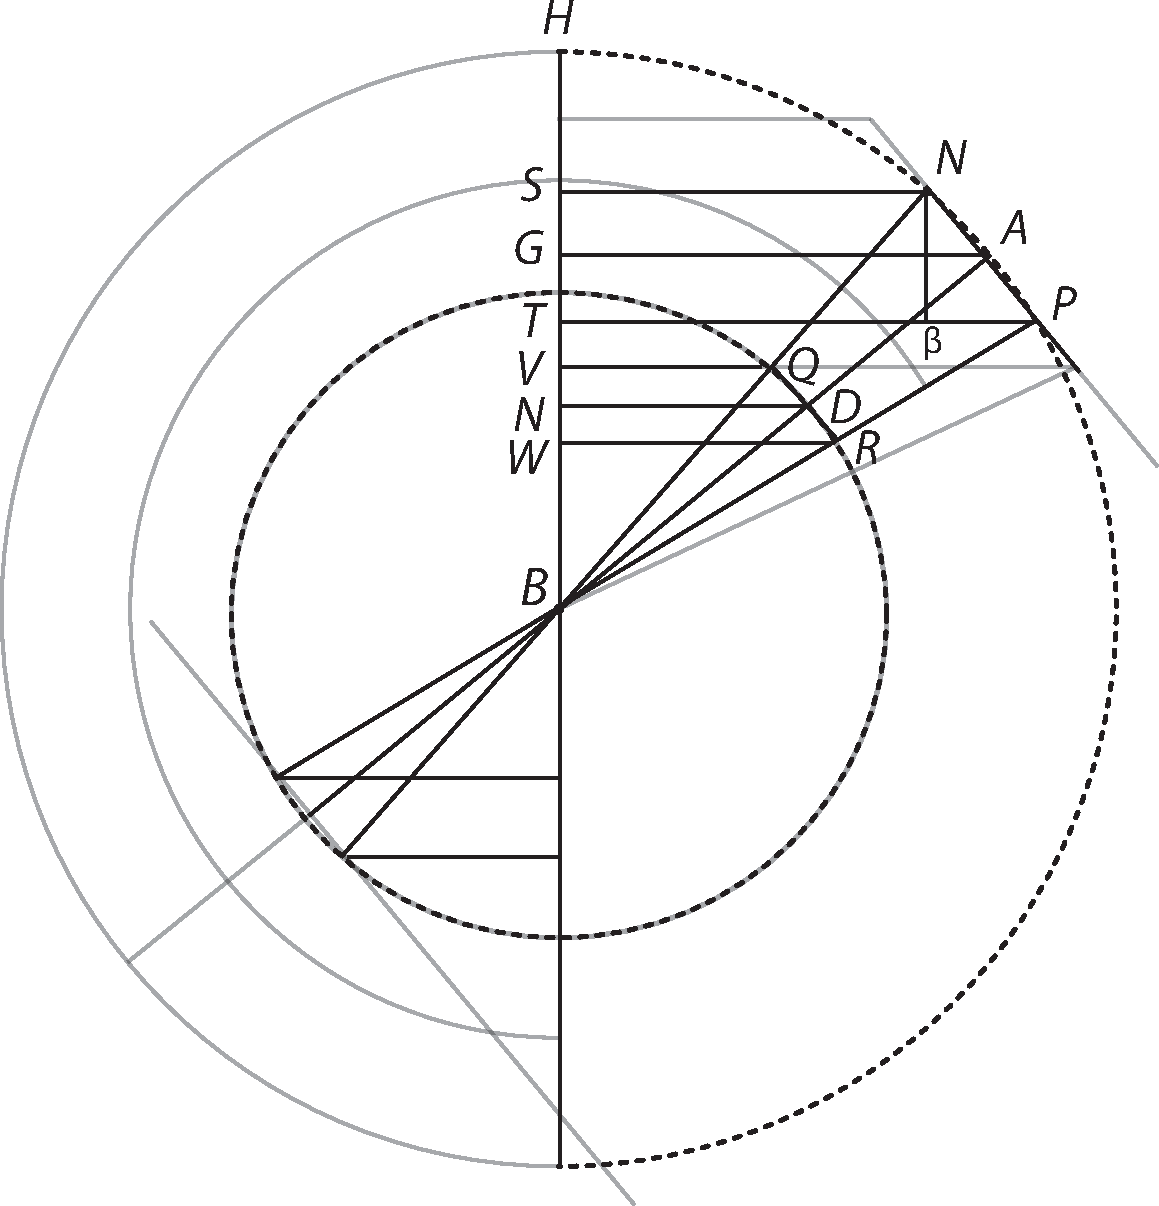
\includegraphics[trim = 0mm -3mm 0mm 0mm, clip, width=0.68\textwidth]{images/LH035,14,02_114v-d4.pdf}\\
\noindent \centering [\textit{Fig. 13, tlw. Blindzeichnung}]\edtext{}{\lemma{\hspace{2mm}[\textit{Fig. 13}]}\killnumber\Cfootnote{Die Bezeichnung $\displaystyle N$ wird für zwei verschiedene Punkte verwendet.}}
\pend
\newpage
%\vspace{1.em}% PR: Rein provisorisch!!
%%%%%%%%%%%%%%%%%%%%
\pstart
(1)%
\protect\index{Sachverzeichnis}{vis ponderis}\textso{
Vis ponderis $\displaystyle A$ descendentis in arcu }%
\edtext{\textso{circuli $\displaystyle A$}}{\lemma{\textso{circuli}}\Bfootnote{%
\textit{(1) }\ $\displaystyle AC$
\textit{(2) }\ $\displaystyle A$
\textit{ L}}}\textso{,
est ad vim ponderis ejusdem descendentis in recta $\displaystyle GB$,
ut est }%
\edtext{\textso{sinus rectus}}{\lemma{\textso{sinus rectus}}\Bfootnote{\textit{erg. L}}}\textso{ %
$\displaystyle AG$ ad }%
\edtext{\textso{radium}}{\lemma{\textso{radium}}\Bfootnote{\textit{erg. L}}}\textso{ %
$\displaystyle AB.$ }%
Est enim vis ponderis descendentis in recta $\displaystyle NP,$
ad vim ponderis descendentis in
\edtext{recta $\displaystyle ST.$}{\lemma{recta}\Bfootnote{%
\textit{(1) }\ $\displaystyle QR.$
\textit{(2) }\ $\displaystyle ST.$
\textit{ L}}}
ut recta $\displaystyle ST$
\edtext{vel $\displaystyle N\beta$}{\lemma{vel $\displaystyle N\beta$}\Bfootnote{\textit{erg. L}}}
ad rectam $\displaystyle NP$, seu
(:~ob Triangula $\displaystyle AGB$ et $\displaystyle N\beta P$ similia~:)
ut sinus rectus $\displaystyle AG$, ad radium $\displaystyle AB.$
\pend
\pstart
(2)%
\protect\index{Sachverzeichnis}{vis ponderis}\textso{
Vis ponderis descendentis }%
\edtext{\textso{in arcu $\displaystyle D,$
ad vim ponderis\protect\index{Sachverzeichnis}{vis ponderis}}}{\lemma{\textso{in}}\Bfootnote{%
\textit{(1)}\ \textso{recta $\displaystyle QR,$ ad vim ponderis}
\textit{(2)}\ \textso{arcu} [...] \textso{ponderis}
\textit{L}}}\textso{ %
descendentis in arcu $\displaystyle A,$ est ut Radius $\displaystyle BD,$ ad radium $\displaystyle BA,$ }%
\edtext{quoniam sunt [vires]\edtext{}{\lemma{vis}\Bfootnote{\textit{L ändert Hrsg.}}}
ut rectae $\displaystyle QR$ et $\displaystyle NP,$
quae sunt ut rectae $\displaystyle BD, BA.$}{\lemma{quoniam}\Bfootnote{%
\textit{(1)}\ rectae $\displaystyle BE,$ sunt ad rectam $\displaystyle BA$
\textit{(2)}\ sunt [...] $\displaystyle BD, BA$
\textit{ L}}}
\pend
% \newpage% Rein provisorisch!!
\pstart 
(3)%
\edtext{}{\lemma{}\Afootnote{\textit{Am Rand:}
$\displaystyle A \ \sqcap$ vis ponderis in arcu $\displaystyle A.$
$\displaystyle D \ \sqcap$ vis ponderis in arcu $\displaystyle D.$\vspace{-6mm}}}
Vis ponderis\protect\index{Sachverzeichnis}{vis ponderis} in arcu $\displaystyle A,$
demta vi aequalis ponderis in arcu $\displaystyle D,$
est ad vim ponderis in arcu $\displaystyle A,$
ut $\displaystyle DA$ differentia radiorum $\displaystyle BA$ et $\displaystyle BD$ ad
\edtext{radium $\displaystyle BA.$ Nam}{\lemma{radium $\displaystyle BA.$}\Bfootnote{%
\textit{(1)}\ Nam vi ponderis in arcu $\displaystyle A,$ appellata $\displaystyle i,$
\textit{(2)}\ Nam
\textit{L}}}
vis ponderis in
\edtext{arcu $\displaystyle D$ est}{\lemma{arcu $\displaystyle D$}\Bfootnote{%
\textit{(1)}\ erit
\textit{(2)}\ est
\textit{L}}}
ad vim ponderis in
\edtext{arcu $\displaystyle A,$ ut}{\lemma{arcu $\displaystyle A,$}\Bfootnote{%
\textit{(1)}\ seu
\textit{(2)}\ ut
\textit{L}}}  
$\displaystyle BD$ ad $\displaystyle BA.$
\edtext{Ergo vis}{\lemma{Ergo}\Bfootnote{%
\textit{(1)}\ vim
\textit{(2)}\ vis
\textit{L}}}
ponderis in arcu $\displaystyle D$ est
$\displaystyle\sqcap\ \protect\rule[-4mm]{0mm}{10mm}\frac{BD}{BA}\, \smallfrown$
vim pond. in 
\edtext{arcu $\displaystyle A,$
seu $\displaystyle\frac{BD}{BA}\smallfrown A.$}{\lemma{arcu $\displaystyle A,$}\Bfootnote{%
\textit{(1)}\ seu ajo
\textit{(2)}\ seu $\displaystyle\frac{BD}{BA}\smallfrown A.$\,
\textit{L}}}
Ergo
\edtext{$\displaystyle\frac{A-D}{A} \sqcap \frac{\protect\overset{1}{\cancel{A}} - \displaystyle\frac{BD}{BA} \cancel{A}}{\cancel{A}}$. Ergo}{\lemma{$\displaystyle\frac{\protect\overset{1}{\cancel{A}} - \frac{BD}{BA} \cancel{A}}{\cancel{A}}$}\Bfootnote{%
\textit{(1)}\ $\displaystyle\ \sqcap\ $
\textit{(2)}\ . Ergo
\textit{L}}}
\edlabel{35,14,02_114v_1}%%%%
\edtext{}{{\xxref{35,14,02_114v_1}{35,14,02_114v_2}}{\lemma{$\displaystyle A - D \ \sqcap $}\Bfootnote{%
\textbar\, 
$\displaystyle\frac{\cancel{A} \smallfrown BA, - \cancel{A} \smallfrown BD}{\cancel{A} \smallfrown BA}$
\textit{ändert Hrsg.}\
\textbar\
\textit{(1)}\ (4) Si ad pondus $\displaystyle A$ accedat pondus $\displaystyle C,$ et si ad pondus $\displaystyle D$ accedat pondus $\displaystyle E$
\textit{(2)}\ (4) Vis machinae [...] \textso{pondus $\displaystyle E$,}
\textit{L}}}}$\displaystyle A - D \, \sqcap\ \lbrack\frac{A \smallfrown BA,\, - A \smallfrown BD}{BA}\rbrack.$\protect\rule[-4mm]{0mm}{10mm}
\pend
\pstart
(4)
Vis machinae\protect\index{Sachverzeichnis}{vis machinae} ex ponderibus $\displaystyle A$
\edtext{et}{\lemma{et}\Bfootnote{\textit{erg. L}}}
$\displaystyle D$ compositis
\edtext{ut in figura}{\lemma{ut in figura}\Cfootnote{Vgl. die Abbildung [\textit{Fig. 12}] auf S. \pageref{LH35,14,02_114v_ref-1}.}}\edtext{
ad vim liberam ponderis\protect\index{Sachverzeichnis}{vis ponderis} unius,
ut \protect\rule[-4mm]{0mm}{10mm}$\displaystyle\frac{BA - BD}{BA}, \smallfrown \frac{AG}{BA}$.}{\lemma{figura}\Bfootnote{%
\textit{(1)}\ hoc est ad vi
\textit{(2)}\ habet $\displaystyle\frac{BA - BD}{BA}, \smallfrown \frac{AG}{BA}$
\textit{(3)}\ ad vim [...] $\displaystyle \smallfrown \frac{AG}{BA}$.
\textit{L}}}
Nam vis machinae seu $\displaystyle A - D$
\edtext{est $\displaystyle \sqcap\ \frac{BA - BD}{BA}, \smallfrown A$ per 3.}{\lemma{est}\Bfootnote{%
\textit{(1)}\ ad $\displaystyle A$ ut
\textit{(2)}\ $\displaystyle \sqcap\ \frac{BA - BD}{BA}, \smallfrown A$ per 3.
\textit{L}}}
\rule[-4mm]{0mm}{10mm}\edtext{Sed\edtext{}{\lemma{}\Afootnote{\textit{Am Rand:} $\displaystyle L \ \sqcap$ vi liberae ponderis\vspace{-3mm}}}
$\displaystyle \frac{A}{L} \sqcap \frac{AG}{[A]B}$\edtext{}{\lemma{$\displaystyle G$}\Bfootnote{\textit{L ändert Hrsg.}}}}{\lemma{Sed}\Bfootnote{%
\textit{(1)}\ $\displaystyle A\, \sqcap L\,$
\textit{(2)}\ $\displaystyle \frac{A}{L} \sqcap \frac{AG}{[A]B}$
\textit{ L}}}
\edtext{per 1}{\lemma{per 1}\Bfootnote{\textit{erg. L}}}.
Ergo $\displaystyle A\, \sqcap \frac{AG}{AB}L.$
ergo $\displaystyle A - D\, \sqcap\, \frac{BA - BD}{BA} \smallfrown \frac{AG}{AB}L.$
\rule[-4mm]{0mm}{10mm}seu $\displaystyle \frac{A - D}{L} \sqcap \frac{BA - BD}{BA^2} [\smallfrown AG].$\edtext{}{\lemma{$\displaystyle \smallfrown AG$}\Bfootnote{\textit{erg. Hrsg.}}}\rule[-4mm]{0mm}{10mm}
\pend
\pstart 
(5)%
\textso{ Si ad pondus $\displaystyle A$ addatur pondus $\displaystyle C$,
itemque si }%
\textso{[ad]}\edtext{}{\lemma{\textso{ad}}\Bfootnote{\textit{erg. Hrsg.}}}
\textso{oppositum $\displaystyle D$ addatur pondus $\displaystyle E$, }%
\edlabel{35,14,02_114v_2}%%%%
\edtext{\textso{ita ut arcus $\displaystyle AE$ sit quadrans, %
}}{\lemma{\textso{ita} [...] \textso{quadrans}}\Bfootnote{\textit{erg. L}}}%
\protect\index{Sachverzeichnis}{vis machinae}\textso{erit vis machinae ad vim ponderis unius }\protect\index{Sachverzeichnis}{vis ponderis}%
\edtext{\textso{absolutam, seu $\displaystyle\frac{A - D}{L},$ ut }}{\lemma{\textso{absolutam,}}\Bfootnote{%
\textit{(1)}\ \textso{ut}
\textit{(2)}\ \textso{seu} $\displaystyle\frac{A - D}{L},$ \textso{ut}
\textit{L}}}% 
\textso{$\displaystyle\frac{BA - BD}{BA} \smallfrown \frac{GF}{AB}$. }\protect\rule[-4mm]{0mm}{10mm}%
Caeterorum enim omnium ratio eadem,
tantum pro $\displaystyle AG$ ponenda $\displaystyle AG\, +\, FC.$
Sed $\displaystyle AG\, +\, FC \, \sqcap\,  FG.$
Cum enim Triangula $\displaystyle AGB$ et $\displaystyle BFC$ sint similia
(:~\edtext{ob ang. $\displaystyle DBF\, \sqcap\, GBA$,}{\lemma{ob}\Bfootnote{%
\textit{(1)}\ arcum $\displaystyle D$
\textit{(2)}\ ang. $\displaystyle DBF$
\textit{L}}}
et $\displaystyle \sqcap\, BCF$
cum uterque sit ipsi $\displaystyle FBC$ supplemento ad \edtext{rectum~:\phantom(\hspace{-1.2mm})
et latus}{\lemma{rectum~:\phantom(\hspace{-1.2mm}) et}\Bfootnote{%
\textit{(1)}\ unus angulus
\textit{(2)}\ latus
\textit{L}}}
$\displaystyle AB$ lateri $\displaystyle BC$ aequale,
erunt et caetera $\displaystyle AG$ ipsi $\displaystyle BF$
et $\displaystyle GB$ ipsi $\displaystyle FC$ aequales.
Ergo $\displaystyle GF\, \sqcap\, AG + GB\, \sqcap\, AG + FC.$ 
\pend
\pstart 
(6)%
\protect\index{Sachverzeichnis}{rota}\textso{ Rota rigida $\displaystyle ACDE$ inclinationem mutante,
ut pondere }%
\edtext{$\displaystyle A$\textso{ translato in $\displaystyle \gamma,$ et %
}}{\lemma{$\displaystyle A$\textso{ translato in}}\Bfootnote{%
\textit{(1)}\ \textso{$\displaystyle G,$ et}
\textit{(2)}\ \textso{$\displaystyle \gamma,$ et}
\textit{L}}}%
\protect\index{Sachverzeichnis}{pondus}\textso{pondere $\displaystyle C$ translato in $\displaystyle \delta$
(caeterisque consimiliter)
ductisque perpendicularibus $\displaystyle \gamma\phi,$ et $\displaystyle \delta\xi.$
erit vis machinae in situ $\displaystyle A,$
ad vim machinae in situ }\protect\index{Sachverzeichnis}{vis machinae}%
\edtext{\textso{$\displaystyle \gamma,$ ut }}{\lemma{\textso{$\displaystyle \gamma,$}}\Bfootnote{%
\textit{(1)}\ \textso{comme}
\textit{(2)}\ \textso{ut}
\textit{L}}}%
\textso{$\displaystyle GF$ ad $\displaystyle \phi\xi.$}
Hoc facile demonstratu,
caetera enim omnia in valore $\displaystyle A-D,$
nempe \protect\rule[-4mm]{0mm}{10mm}$\displaystyle \sqcap\ \frac{BA - BD}{BA^2} \smallfrown GF$
constantia praeter $\displaystyle GF,$
cujus loco nunc $\displaystyle \phi\xi.$
\pend
\count\Afootins=900
\count\Bfootins=900
\count\Cfootins=900
\pstart 
(7)
Vis continuatione\protect\index{Sachverzeichnis}{vis machinae}
\edtext{motus machinae in quolibet}{\lemma{motus}\Bfootnote{%
\textit{(1)}\ in qualibet
\textit{(2)}\ machinae in quolibet
\textit{L}}}
puncto ut $\displaystyle A$ quaesita,
est ad vim a pondere\protect\index{Sachverzeichnis}{vis ponderis}
$\displaystyle A$ libere cadente in recta $\displaystyle AG$
ex eadem altitudine in respondente puncto $\displaystyle G$
\edtext{quaesitam, quemadmodum}{\lemma{quaesitam,}\Bfootnote{%
\textit{(1)}\ ut
\textit{(2)}\ vel ad vim\ \textbar\ acceleratione \textit{erg.}\ \textbar\ quaesitam in alio puncto ut $\displaystyle \gamma.$
\textit{(3)}\ quemadmodum
\textit{L}}} 
sunt [vires]\edtext{}{\lemma{vis}\Bfootnote{\textit{L ändert Hrsg.}}} simplices,\protect\index{Sachverzeichnis}{vis simplex}
% [ut]\edtext{}{\lemma{}\Bfootnote{ut \textit{erg. Hrsg.}}}
pendet ex demonstratis paulo ante.
Tantum notandum
\edtext{est si pondus $\displaystyle A$}{\lemma{est}\Bfootnote{%
\textit{(1)}\ quoties pondus $\displaystyle A$
\textit{(2)}\ percurrant ei
\textit{(3)}\ si pondus $\displaystyle A$
\textit{L}}}
succedaneo ita suppleatur,
ut machina\protect\index{Sachverzeichnis}{machina} semper in eodem servetur statu,
punctum respondens $\displaystyle G$ vel $\displaystyle \phi$
non in recta $\displaystyle HB,$
sed in proxima $\displaystyle BL,$
aut tertia $\displaystyle L\lambda,$
\edtext{aliaque numeri percursionum}{\lemma{aliaque}\Bfootnote{%
\textit{(1)}\ toties 
\textit{(a)}\ continuatur,
\textit{(b)}\ producta, quot
\textit{(2)}\ numero percursionum
\textit{(3)}\ numeri percursionum
\textit{L}}}
ipsius arcus $\displaystyle H\psi$ numero respondentis
quaerendum est,
nempe si secunda est revolutio in secunda recta $\displaystyle BL,$
si tertia, in tertia.
Et punctum sumtum
\edtext{ut $\displaystyle G$}{\lemma{ut $\displaystyle G$}\Bfootnote{\textit{erg. L}}}
in $\displaystyle BL$ vel $\displaystyle L\lambda,$
tantum aberit a $\displaystyle B$ vel $\displaystyle \lambda,$
quantum respondens ei $\displaystyle G$ vel $\displaystyle \phi$ ab $\displaystyle H.$
Quae ergo illo in puncto in recta $\displaystyle HG$ vel ejus continuata sumto.
%
[115~r\textsuperscript{o}] %%%%%%%%%% HIER BEGINNT BLATT 115r.
%
Non licet autem diversa inter se conferre puncta, hoc modo
et dicere vim acceleratione\protect\index{Sachverzeichnis}{acceleratio}
quaesitam in puncto $\displaystyle A$ esse ad eam quae in puncto $\displaystyle\gamma$
ut [vires]\edtext{}{\lemma{vis}\Bfootnote{\textit{L ändert Hrsg.}}} simplices:
ratio disparitatis, \edtext{quia
vires}{\lemma{quia}\Bfootnote{%
\textit{(1)}\ vis
\textit{(2)}\ vires
\textit{L}}}
simplices\protect\index{Sachverzeichnis}{vis simplex}
in punctis $\displaystyle A$ vel $\displaystyle\gamma,$
conferendae ad eandem potentiam
\edtext{liberam simplicem}{\lemma{liberam}\Bfootnote{%
\textit{(1)}\ rectae
\textit{(2)}\ simplicem
\textit{L}}};
sed non acquisitae in punctis $\displaystyle A$ et $\displaystyle\gamma$
ad eandem  liberam acquisitam,
sed ad diversas, nempe in respondentibus punctis.
\pend
\pstart
(8)
Vis acceleratione\protect\index{Sachverzeichnis}{acceleratio}
gravis\protect\index{Sachverzeichnis}{vis gravis} descendentis quaesita
tanta est, ut possit grave restituere in altitudinem ex qua delapsum est;
si medium\protect\index{Sachverzeichnis}{medium} non obstet.
Hoc facile demonstratur.
Restituet scilicet in altitudinem priore minorem intervallo minore quolibet dato,
perditis continue accelerationis incrementis.
\pend
\pstart
(9)
Hinc sequitur[,]
\edtext{si non obstet medium simplici gravitate\protect\index{Sachverzeichnis}{gravitas} sequi
motum perennem\protect\index{Sachverzeichnis}{motus perennis}.}{\lemma{si}\Bfootnote{%
\textit{(1)}\ grave
\textit{(2)}\ non obstet medium 
\textit{(a)}\ fieri per gravitatem, ut motus
\textit{(b)}\ simplici gravitate
\textit{(aa)}\ motum pe
\textit{(bb)}\ omnia in statum pri
\textit{(cc)}\ sequi motum perennem.
\textit{L}}}
\pend
\pstart
(10)
Hinc sequitur vim acceleratione\protect\index{Sachverzeichnis}{acceleratio}
gravis\protect\index{Sachverzeichnis}{vis gravis} descendentis quaesitam
tantam esse, ut omnia restituere possit in statum
restitutioni\protect\index{Sachverzeichnis}{restitutio} gravis aequivalentem;
aequivalentem autem voco,
qui tantundem motus producat;
orti a gravitate.\protect\index{Sachverzeichnis}{gravitas}
Magnitudinem autem \edtext{motus\protect\index{Sachverzeichnis}{magnitudo motus}
aestimandam patet,}{\lemma{motus}\Bfootnote{%
\textit{(1)}\ aestimandam arbitror
\textit{(2)}\ aestimandam patet
\textit{L}}}
ex ductu celeritatis\protect\index{Sachverzeichnis}{celeritas} in corpus.
\pend
\pstart
(11)
Corporis gravis\protect\index{Sachverzeichnis}{vis gravis}
\edtext{cadentis}{\lemma{ cadentis}\Bfootnote{\ \textit{erg. L}}}
tanta \edtext{prorsus}{\lemma{ prorsus}\Bfootnote{\ \textit{erg. L}}}
vis est, \edtext{ut catenam}{\lemma{ ut}\Bfootnote{%
\textit{(1)}\ cylindrum
\textit{(2)}\ catenam
\textit{L}}}
corporum similium
\edtext{et similiter positorum}{\lemma{}\Bfootnote{et similiter positorum\ \textit{erg. L}}}
et aequalium contiguorum,
in eam possit altitudinem attollere
quae sufficiat ad motum similem et aequalem perpetuo continuandum.%
\pend
\pstart
Unde sequitur motum perpetuum\protect\index{Sachverzeichnis}{motus perpetuus}
ope ictus\protect\index{Sachverzeichnis}{ictus} ejusmodi haberi non posse,
ut visum est doctissimo Viro,
\edtext{qui machinae\protect\index{Sachverzeichnis}{machina} cujusdam ad eam rem pertinentis descriptionem}{\lemma{qui}\Bfootnote{%
\textit{(1)}\ ejus rei d
\textit{(2)}\ machinae [...] descriptionem
\textit{L}}}\edtext{
sub finem \textit{Cursus Mathematici}
patris Schotti\protect\index{Namensregister}{\textso{Schott} (Schottus), Kaspar 1608-1666}
dedit.}{\lemma{descriptionem [...] dedit}\Cfootnote{\cite{00093}K. \textsc{Schott}, \textit{Cursus mathematicus}, Würzburg 1661, S. 655f.}}
Cujus tamen propositio mihi [inveniendi]\edtext{}{\lemma{inveniendae}\Bfootnote{\textit{L ändert Hrsg.}}}
tam \edtext{insignis theorematis}{\lemma{insignis}\Bfootnote{%
\textit{(1)}\ proprietatis
\textit{(2)}\ theorematis
\textit{L}}},
\edtext{quo vis accelerationis\protect\index{Sachverzeichnis}{vis accelerationis}}{\lemma{quo}\Bfootnote{%
\textit{(1)}\ vis gravium\protect\index{Sachverzeichnis}{vis gravis} ad regulam
\textit{(2)}\ vis accelerationis
\textit{L}}}
perfecte aestimari potest, occasionem
\edtext{dedit. Clarus}{\lemma{dedit.}\Bfootnote{%
\textit{(1)}\ Ingeniosissimus
\textit{(2)}\ Clarus
\textit{L}}}
Mariottus\protect\index{Namensregister}{\textso{Mariotte}, Edme, Seigneur de Chazeuil ca. 1620-1684},\hfill 
vir\hfill  in\hfill  experimentis\hfill  indagandis\hfill  et\hfill  explicandis\hfill  ingeniosae\hfill felicitatis,
\pend
\newpage% Rein provisorisch
%%%%%%%%%%%%%%%%%%%% PR: Bitte, Abbildungen korrekt setzen. Danke.
%\vspace*{1.5em}
\count\Afootins=1200
\count\Bfootins=1200
\count\Cfootins=1200
\pstart
\noindent
\centering
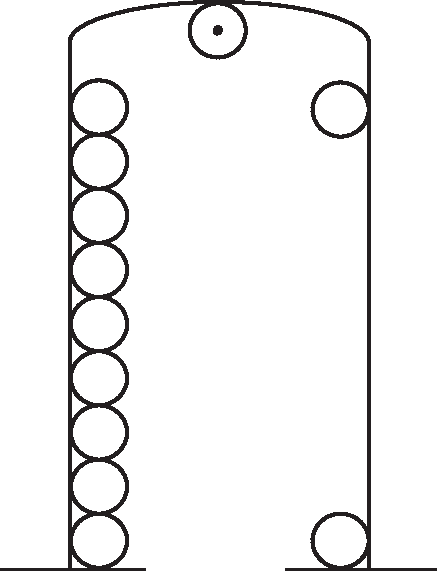
\includegraphics[trim = 0mm -3mm 0mm 0mm, clip, width=0.3\textwidth]{images/LH035,14,02_115r-d1.pdf}\\
\noindent \centering [\textit{Fig. 14}]
\pend
\vspace{1.5em}
%%%%%%%%%%%%%%%%%%%%
\pstart
\noindent\setline{1}\edtext{observavit aliquando
guttae lapsu sustineri circiter cylindrum aquae
aequalis cum gutta latitudinis et ejus altitudinis
quanta est ex qua delapsa est \edtext{gutta.\protect\index{Sachverzeichnis}{gutta}
Unde}{\lemma{gutta.}\Bfootnote{%
\textit{(1)}\ Sed
\textit{(2)}\ Unde
\textit{L}}}
ille concludit vim gravis accelerati esse ponderi ejusmodi cylindri aequalem.}{\lemma{observavit [...] aequalem}\Cfootnote{%
\cite{00311}E. \textsc{Mariotte}, \textit{De la percussion}, Paris 1673, S. 210ff.}}
Verum fatendum est inter \edtext{pondus\protect\index{Sachverzeichnis}{pondus}
seu vim ut vocare soleo mortuam,\protect\index{Sachverzeichnis}{vis mortua}
et}{\lemma{pondus}\Bfootnote{%
\textit{(1)}\ et
\textit{(2)}\ seu vim [...] mortuam, et
\textit{L}}}
vim acceleratione quaesitam nullam esse posse rationem;
non magis quam inter
\edtext{lineam et superficiem}{\lemma{lineam et}\Bfootnote{%
\textit{(1)}\ corpus
\textit{(2)}\ spatium
\textit{(3)}\ superficiem
\textit{L}}};
et \edtext{ut recte animadversum est a
Galilaeo\protect\index{Namensregister}{\textso{Galilei} (Galilaeus, Galileus), Galileo 1564-1642}
et demonstratum ab ejus discipulis
Joh. Alphonso Borello\protect\index{Namensregister}{\textso{Borelli} (Borellus), Giovanni Alfonso 1608-1679}
aliisque et vero ex ipsis
Galilaei\protect\index{Namensregister}{\textso{Galilei} (Galilaeus, Galileus), Galileo 1564-1642}
traditis \edtext{manifestum; lapsu corporis%
}{\lemma{manifestum;}\Bfootnote{%
\textit{(1)}\ vim corporis
\textit{(2)}\ lapsu corporis
\textit{L}}}
quantulicunque aliud quantumcunque non tantum sustineri aliquandiu,
sed et in aliquam altitudinem attolli posse.}{\lemma{ut [...] posse}\Cfootnote{
Neben \cite{01001}G.~A. \textsc{Borelli}, \textit{De vi percussionis}, Bologna 1667, bes. Kap. 27-29, dürfte Leibniz auch Kenntnis von Galileis Abhandlung \textit{Le mecaniche} in der französischen Übersetzung von Marin Mersenne gehabt haben, deren letztes (11.) Kapitel gänzlich dem Thema \textit{De la force de la percussion} gewidmet ist. Siehe \cite{01091}G. \textsc{Galilei}, \textit{Les mechaniques}, Paris 1634, S. 69-73.
}}
\pend
\pstart
Nec vero necesse est supponere
ut vis ipsa parvitatis primae sit instar
\edtext{puncti; est enim instar lineae infinite parvae,
ad lineam communem. Aut}{\lemma{puncti;}\Bfootnote{%
\textit{(1)}\ est enim instar lineae sed in
\textit{(2)}\ est [...] parvae,
\textit{(a)}\ aut
\textit{(b)}\ ad [...] Aut
\textit{L}}}
potius si mavis instar lineae ad superficiem:
Etsi interim alia atque alia ipsa quoque esse possit,
pro diversa vi \edtext{quam
causa gravitatis\protect\index{Sachverzeichnis}{causa gravitatis}}{\lemma{quam}\Bfootnote{%
\textit{(1)}\ grave
\textit{(2)}\ causa gravitatis
\textit{L}}} habet,
sive ea a motu aetheris,\index{Sachverzeichnis}{aether}
sive ab alio denique principio oriatur:
quemadmodum ventus\index{Sachverzeichnis}{ventus} et remi accelerationem conferunt navi.
\pend
\count\Afootins=1200
\count\Bfootins=1200
\count\Cfootins=1200
\pstart
\edtext{Tantum supponendum est}{\lemma{Tantum}\Bfootnote{%
\textit{(1)}\ ad dem
\textit{(2)}\ supponendum est
\textit{L}}}
causam gravitatis\protect\index{Sachverzeichnis}{causa gravitatis} ita agere,
ut quolibet momento, seu tempore minore quam quod assignabile est[,]
novum inferat ictum.\protect\index{Sachverzeichnis}{ictus}
Nam si intra certum temporis spatium, finitus sit ictuum numerus
quemadmodum \edtext{de vento et remis}{\lemma{de}\Bfootnote{%
\textit{(1)}\ tempore
\textit{(2)}\ vento et remis
\textit{L}}} manifestum est;
tunc calculo aestimare facile est,
quam rationem habeat
\edtext{vis quaesita acceleratione\protect\index{Sachverzeichnis}{acceleratio},
ad}{\lemma{vis}\Bfootnote{%
\textit{(1)}\ celeritate\protect\index{Sachverzeichnis}{celeritas} quaesita ad
\textit{(2)}\ quaesita acceleratione, ad
\textit{L}}}
ictum \edtext{primum.
Haec}{\lemma{primum.}\Bfootnote{%
\textit{(1)}\ Sed
\textit{(2)}\ Haec
\textit{L}}}
dicenda essent in \edtext{Hypothesi
Gassendi,\protect\index{Namensregister}{\textso{Gassendi} (Gassendus), Pierre 1592-1655}
\protect\index{Namensregister}{\textso{Demokrit} von Abdera 2. H. 5. Jh. v. Chr.}\edtext{Democriti.}{\lemma{Democriti}\Bfootnote{\textit{erg. L}}}}{\lemma{Hypothesi Gassendi, Democriti}\Cfootnote{Damit ist offenbar der Atomismus gemeint. Zur Ursache der Schwere und der Beschleunigung fallender Körper insbesondere siehe P. \textsc{Gassendi}, \textit{Physica}, sectio I, lib. V, cap. II-III\cite{01073} (\textit{GOO} I, S. 343a-350a).\cite{01029}}}
Sed si \edtext{cum Aristotele\protect\index{Namensregister}{\textso{Aristoteles}, 384-322 v. Chr.},
fluidum et continuum aethera\protect\index{Sachverzeichnis}{aether}
supponamus}{\lemma{cum Aristotele [...] supponamus}\Cfootnote{\textsc{Aristoteles}, \textit{De caelo} I 3.\cite{00303} Aristoteles beschreibt den Äther aber nicht als ein Fluidum.}};
\edtext{ejusque motui sive conatui\protect\index{Sachverzeichnis}{conatus}
causam tribuamus gravitatis\protect\index{Sachverzeichnis}{causa gravitatis}
sive cum Cartesio\protect\index{Namensregister}{\textso{Descartes} (Cartesius, des Cartes), Ren\'{e} 1596-1650}
\edtext{a vortice\protect\index{Sachverzeichnis}{vortex}}{\lemma{a}\Bfootnote{%
\textit{(1)}\ motu terrae, sive
\textit{(2)}\ vortice
\textit{L}}} quodam
}{\lemma{ejusque [...] quodam}\Cfootnote{R. \textsc{Des\-cartes}, \textit{Principa philosophiae}, IV, §~20-27, Amsterdam 1644, S.~199-204\cite{00035} (\textit{DO} VIII.A, S.~212-217\cite{00120}).}}\edtext{sive \edtext{ex sententia nostra}{\lemma{ex sententia nostra}\Cfootnote{Siehe etwa \cite{01071}\textit{LSB} VI, 3 N.~2\textsubscript{1}, S.~6; N.~2\textsubscript{3}, Prop. 10, S.~22-26.
Erste Ansätze finden sich in der \textit{Hypothesis physica nova} von 1671. Siehe \cite{00256}\textit{LSB} VI, 2 N.~40, S.~223-228.}}}{\lemma{quodam sive}\Bfootnote{%
\textit{(1)}\ mecum
\textit{(2)}\ ex sententia nostra
\textit{L}}}
a luminis motu causam petamus,
ne scilicet ubi ex \edtext{cognitis
phaenomenis ratio}{\lemma{cognitis}\Bfootnote{%
\textit{(1)}\ ratio
\textit{(2)}\ phaenomenis ratio
\textit{L}}}
reddi potest,
ad \edtext{Hypothesin
arbitrariam confugiamus}{\lemma{Hypothesin}\Bfootnote{%
\textit{(1)}\ confugere necesse sit
\textit{(2)}\ arbitrariam confugiamus
\textit{L}}}[,]
sequitur continuam esse gravitatis causam;\protect\index{Sachverzeichnis}{causa gravitatis}
adeoque et Galilaei\protect\index{Namensregister}{\textso{Galilei} (Galilaeus, Galileus), Galileo 1564-1642}
hypothesin veram \edtext{esse.
Quicquid sit etsi}{\lemma{esse.}\Bfootnote{%
\textit{(1)}\ Quae etsi ver
\textit{(2)}\ Quicquid sit
\textit{(a)}\ ea
\textit{(b)}\ si
\textit{(c)}\ non
\textit{(d)}\ etsi 
\textit{L}}}
continua non foret,
continuae adeo ex adversa sententia futura est
\edtext{similis, ut
ictibus\protect\index{Sachverzeichnis}{ictus} in}{\lemma{similis, ut}\Bfootnote{%
\textit{(1)}\ in
\textit{(2)}\ ictus
\textit{(3)}\ ictibus in
\textit{L}}}
quolibet tempore longe minore
quam sit sensibile quodlibet datum
\edtext{repetitis ut
in usu vitae}{\lemma{repetitis ut}\Bfootnote{%
\textit{(1)}\ ad sensum
\textit{(2)}\ ad senten
\textit{(3)}\ in usu vitae
\textit{L}}}
hypothesis Galilaei\protect\index{Namensregister}{\textso{Galilei} (Galilaeus, Galileus), Galileo 1564-1642}
pro vera haberi possit,
quemadmodum in staticis horizontalem esse planum;
et in Opticis radios solis esse parallelos.
\pend
\pstart
Superest ergo insignis indagatio,
de altitudine ad quam pendula\protect\index{Sachverzeichnis}{pendulum} assurgunt:
Videndumque est an regula condi possit,
cujus ope data penduli longitudine et ponderis gravitate definiatur altitudo.
\pend
%\vspace{1.0em}
\newpage
\pstart%
\noindent%
[\textit{Marginalie auf Bl. 114~v\textsuperscript{o}:}]
\pend
\vspace{0.5em}%
\pstart%
\noindent%
$\displaystyle y + \sqrt{\protect\phantom{a^2 + y^2}}\hspace*{-10,3mm}a^2 \pPsMs\, y^2\ \sqcap\ x.$\edtext{ %
$\displaystyle\ \sqrt{\protect\phantom{a^2 + y^2}}\hspace*{-10,3mm}a^2 \pPsMs\, y^2\ \sqcap\ x -y.\ $}{\lemma{$\displaystyle\sqcap\ x.$}\Bfootnote{%
\textit{(1)}\ Ergo $\displaystyle y$
\textit{(2)}\ $\displaystyle \sqrt{\protect\phantom{a^2 + y^2}}\hspace*{-9mm}a^2 \pPsMs\, y^2\ \sqcap\ x -y$
\textit{L}}}
Ergo $\displaystyle a^2 \pPsMs\, y^2 \, \sqcap \ x^2 -2yx + y^2.\ $
Unde si $\displaystyle \pPsMs \ \sqcap\ +$
ut in Hyperbola fiet:
\protect\rule[-4mm]{0mm}{10mm}$\displaystyle a^2 \, \sqcap \ x^2 - 2yx.\ $
sive $\displaystyle \frac{- a^2 + x^2}{2x}\, \sqcap \ y.\ $
In circulo fiet:
$\displaystyle a^2 - 2y^2 + 2yx \, \sqcap \, x^2.\ $
Quaerenda est
\edtext{maxima $\displaystyle x.$ ordinetur:}{\lemma{maxima}\Bfootnote{%
\textit{(1)}\ tangens
\textit{(2)}\ $\displaystyle x.$
\textit{(a)}\ quaeratur
\textit{(b)}\ ordinetur
\textit{L}}}
\quad$\displaystyle x^2 - 2yx$\quad$\displaystyle -2y^2 + 2yx.\ $\
vel $\displaystyle\ \cancel{2}xl - \cancel{2}yl \ \sqcap\, \overset{2}{-\cancel{4}} y^2 + \cancel{2}yx.\ $
et erit \protect\rule[-4mm]{0mm}{10mm}$\displaystyle l \, \sqcap \frac{-2y^2 + yx}{x- y}.\ $
sive $\displaystyle l \, \sqcap \frac{- \raisebox{-2.55mm}{{\def\firstcircle{(0,0) circle (0.35cm)}\begin{tikzpicture}\draw \firstcircle node {$2$};\end{tikzpicture}}} y^2 \raisebox{-2.55mm}{{\def\firstcircle{(0,0) circle (0.35cm)}\begin{tikzpicture}\draw \firstcircle node {$+y^2$};\end{tikzpicture}}} + y \sqrt{a^2-y^2}}{\sqrt{a^2 - y^2}} \sqcap \frac{-y^2}{\sqrt{a^2-y^2}} + y.\ $\edtext{
divide}{\lemma{$\displaystyle +\ y$}\Bfootnote{%
\textit{(1)}\ quando
\textit{(2)}\ divide
\textit{L}}}
$\displaystyle l$ per
[$\displaystyle y$]\edtext{}{\lemma{$\displaystyle y$}\Bfootnote{\textit{erg. Hrsg.}}}
et multiplica per \protect\rule[-4mm]{0mm}{10mm}$\displaystyle \sqrt{a^2 - y^2},\ $
fiet: $\displaystyle - y + \sqrt{a^2 - y^2}.\ $
quam formulam pone $\displaystyle \sqcap\ 0.$
et \edtext{habebis $\displaystyle l$ infinite parvam}{\lemma{habebis}\Bfootnote{%
\textit{(1)}\ maximam
\textit{(2)}\ $\displaystyle l$ infinite parvam
\textit{L}}}
seu \edtext{verticem figurae,}{\lemma{verticem figurae}\Cfootnote{Vgl. die Abbildung [\textit{Fig. 15}].}}
%auf S. \pageref{LH035,14,02_114v-ref2}.}}
sin ponas divisorem $\displaystyle \sqcap\ 0.$
erit $\displaystyle l$ infinita,
ergo tunc $\displaystyle a\, \sqcap\, y.\ $
$\displaystyle y + \sqrt{a^2 - y^2} \sqcap x.\ $
seu $\displaystyle a^2 - y^2 \sqcap x^2 - 2yx + y^2.\ $\protect\rule[-4mm]{0mm}{10mm}
Quaeritur $\displaystyle x$ 
\edtext{maxima: ordinetur}{\lemma{maxima:}\Bfootnote{%
\textit{(1)}\ determinetur
\textit{(2)}\ ordinetur
\textit{L}}}
2\textsuperscript{dum}
\hspace*{-3,mm}
$\displaystyle%
\begin{array}{l}
x.\ \text{fiet:}\\
\\
\\
\\
\end{array}$%
$\displaystyle%
\begin{array}{ccc}
x^2 & - 2yx & + 2y^2.\\
& & -a^2\\
2 & 1 & 0\\
\hline \cancel{2}x \cancel{^2} & - \cancel{2}y \cancel{x} \ \sqcap & 0
\end{array}$%
$\displaystyle%
\begin{array}{l}
\text{Ergo}\ x \, \sqcap \, y.\ \text{Ergo [\textit{Text bricht ab.}]}\\
\\
\\
\\
\end{array}$
\pend
\pstart
\setline{11}
\vspace*{2.0em}
\noindent
\centering
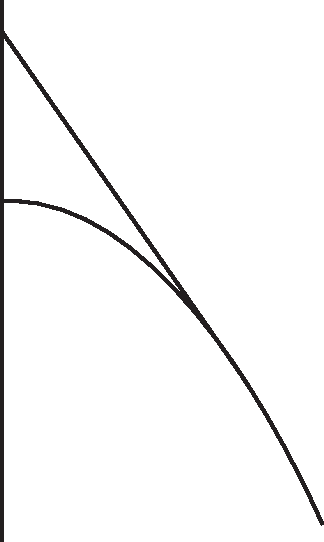
\includegraphics[trim = 0mm -3mm 0mm 0mm, clip, width=0.15\textwidth]{images/LH035,14,02_114v-d5.pdf}\\
\noindent \centering [\textit{Fig. 15}]\label{LH035,14,02_114v-ref2}
\pend
\count\Afootins=1500
\count\Bfootins=1500
\count\Cfootins=1500
%
%%%%%%%%%% HIER ENDET DAS STÜCK. 